\section{実験装置}
用いる実験装置は、光検出デバイスMPPC、MPPC読み出しモジュールEASIROC、暗箱、光学機器、スリット、しぼり、LED。光学機器を図のように並べ、光の干渉を起こす。各デバイスの位置や距離によって干渉の見え方が変わるが、これは実際に物を置いていろいろ試してみるとよい。以下では、光検出器とその読み出しについて説明する。
\begin{figure}[h]
\begin{center}
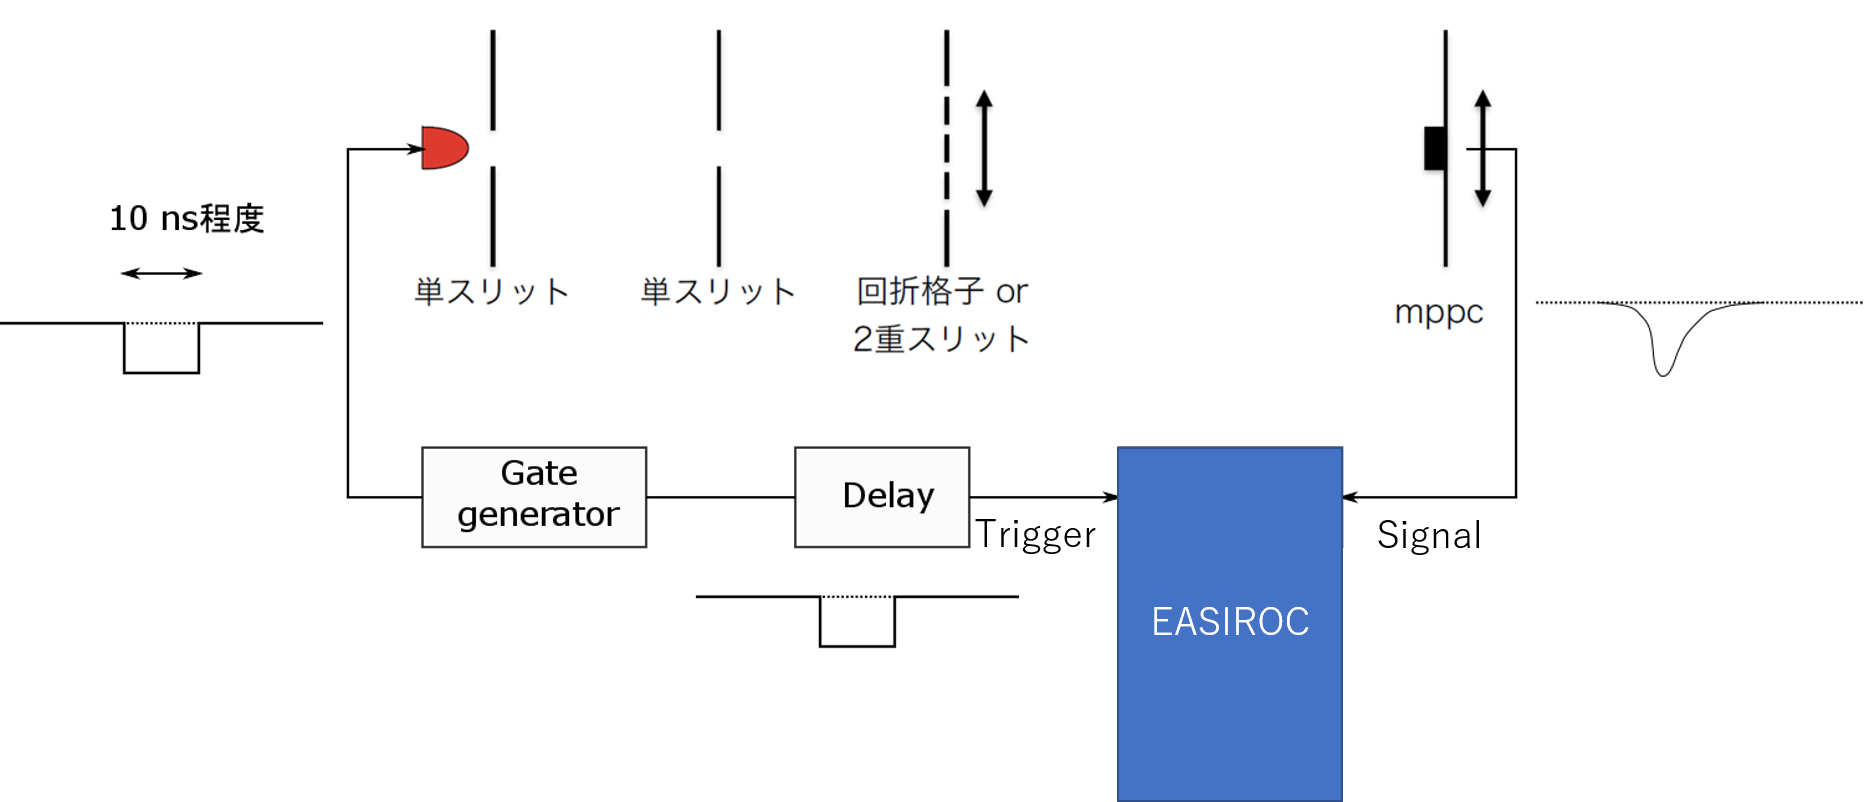
\includegraphics[width=12cm]{setup.png}
\end{center}
\caption{セットアップ}
\end{figure}
\subsection{MPPC}
MPPC(Micro Pixel Photon Counter)はAvalamche Photo Diode(APD)が多数配列された光検出器である。APDは半導体でできている。P型とN型、異なるドープ型の半導体にある向きで電圧をかけると、キャリアの少ない空乏層ができる。ここに光子が入射すると、光電効果で電子をはじき出す。電子は印加電圧によってエネルギーを持ち、さらに周囲の原子殻内電子をはじき出し、雪崩(Avalanche)的に電子を倍増する。印加電圧によって様々な倍増モードがあるが、MPPC内のAPDでは、十分な印加電圧をかけることで入射光子数によらない出力電流を得る(ガイガーモード)。このガイガーモードAPDが多数配列することにより、我々は光子が入射したAPDのチャンネル数だけを数えることで、(pile upはあるものの)光子数をデジタルに数えることができる。
\begin{figure}[h]
\begin{tabular}{ccc}
\begin{minipage}[t]{0.33\hsize}
\begin{center}
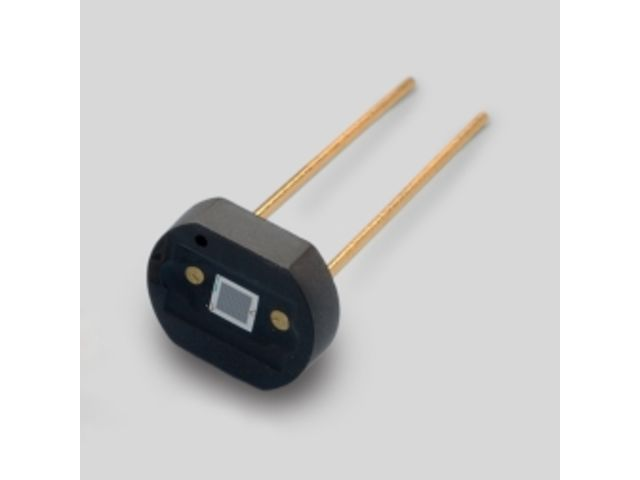
\includegraphics[width=4cm]{mppc.jpg}
\end{center}
\caption{MPPC}
\end{minipage}
\begin{minipage}[t]{0.33\hsize}
\begin{center}
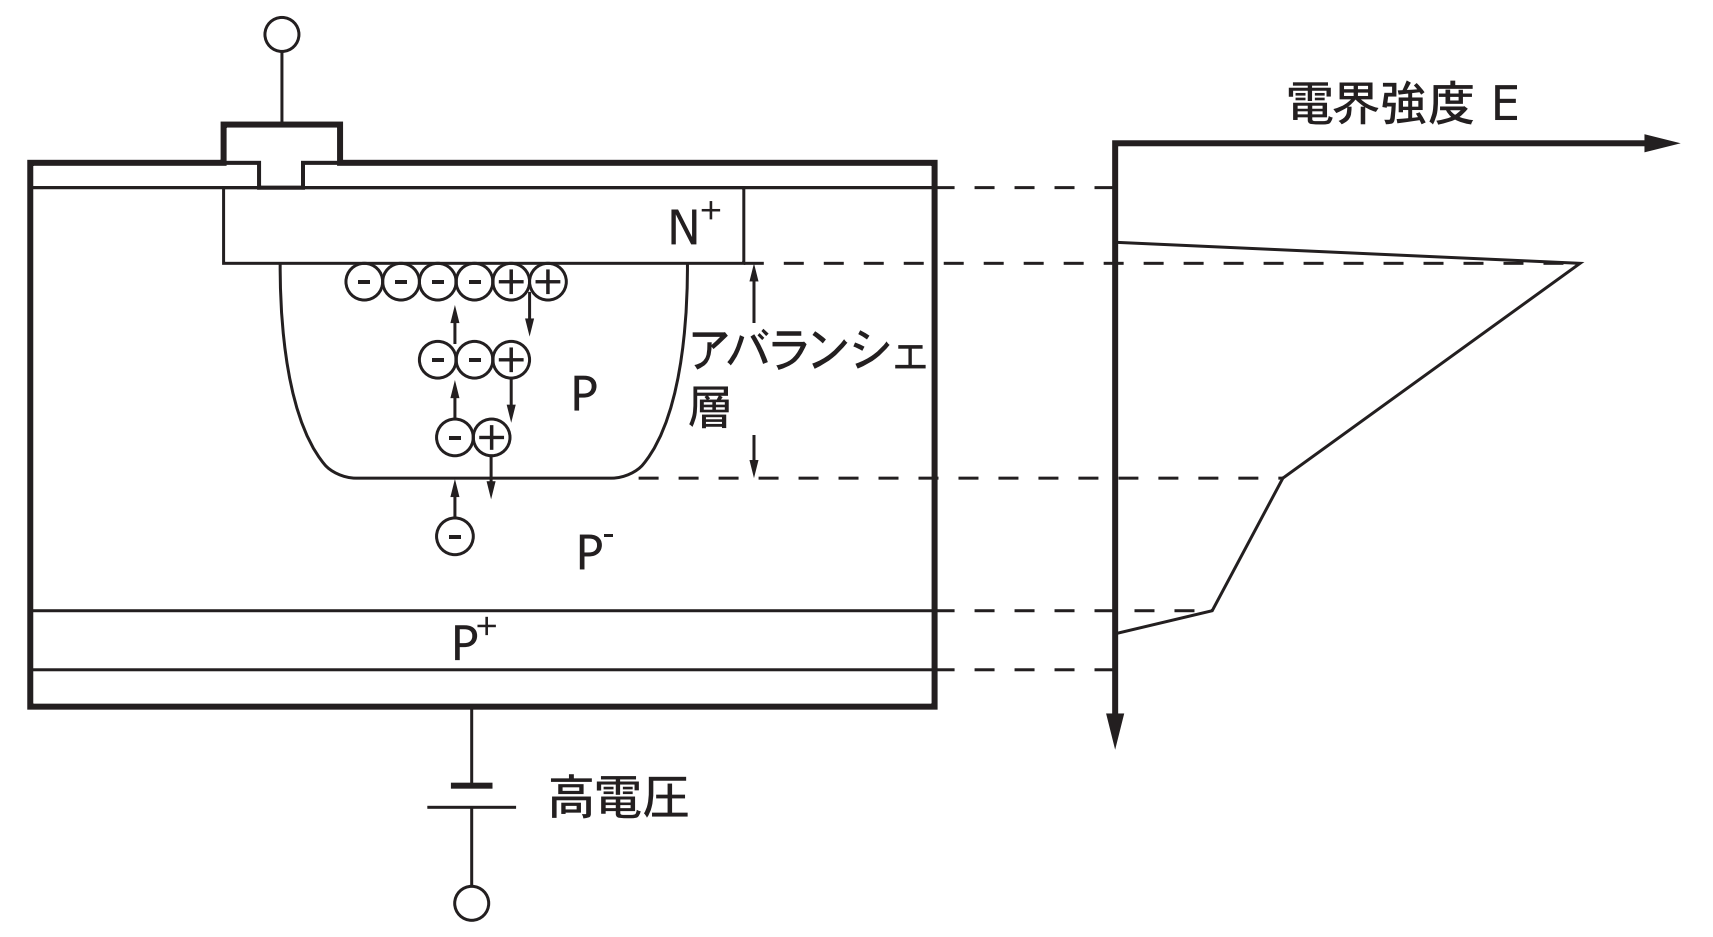
\includegraphics[width=4cm]{APDstructure.PNG}
\end{center}
\caption{APD}
\end{minipage}
\begin{minipage}[t]{0.33\hsize}
\begin{center}
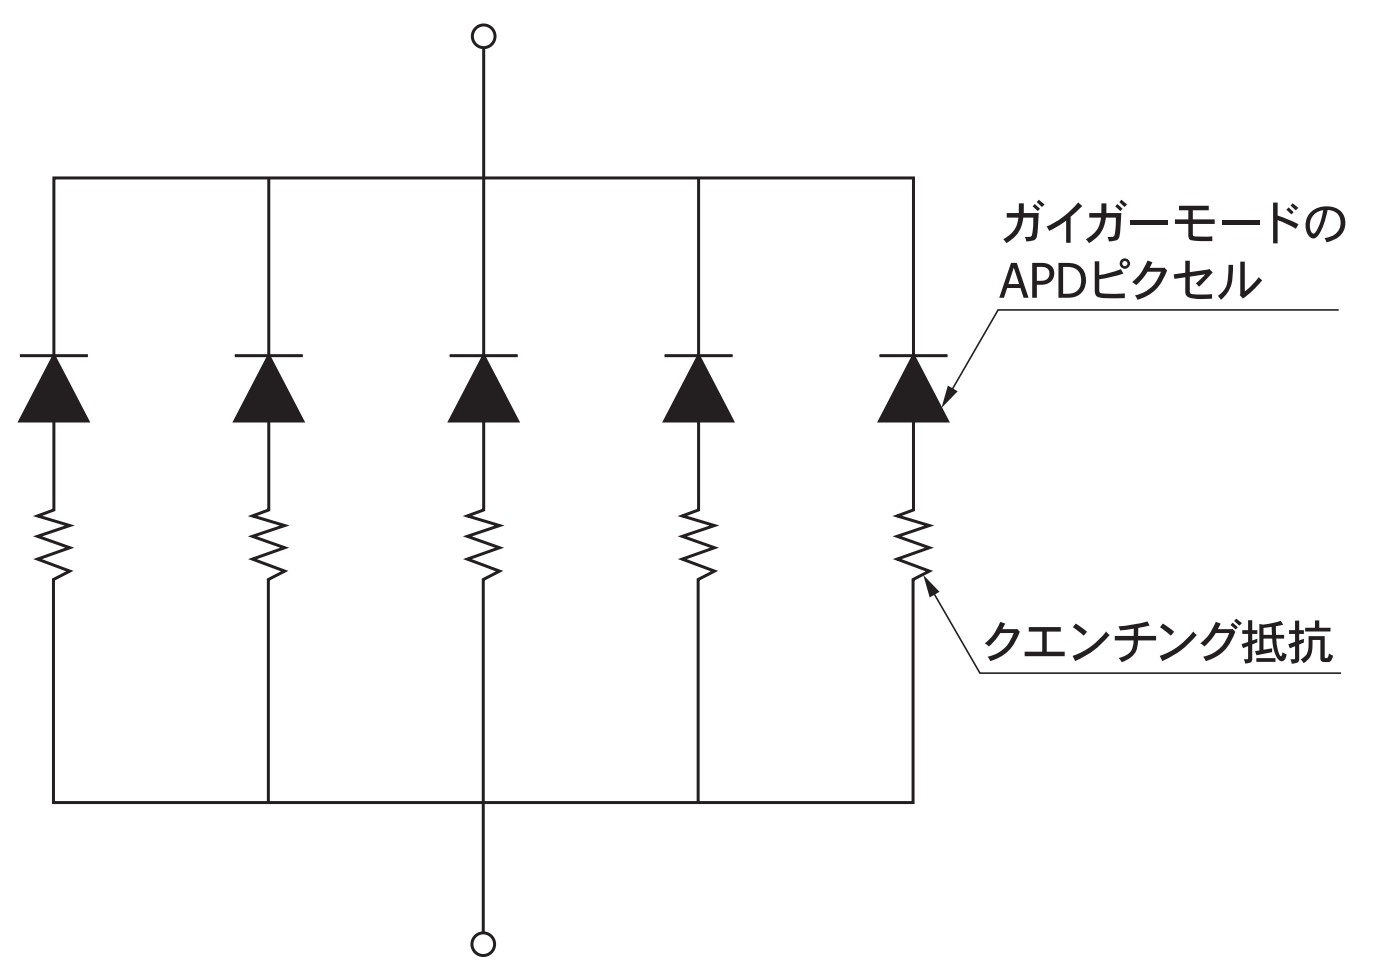
\includegraphics[width=4cm]{QuenchingArray.PNG}
\end{center}
\caption{MPPCはAPDを並列に並べたもの}
\end{minipage}
\end{tabular}
\end{figure}
浜松ホトニクスのハンドブックに、詳細なMPPCの挙動が説明されている。\cite{hamamatsu}
\subsection{EASIROC}
EASIROCモジュールは、書き換え不可能な集積回路(ASIC)であるEASIROCチップと、EASIROCチップ制御用の書き換え可能な集積回路(FPGA)であるArtix7が搭載された、MPPCの(多チャンネネル)読み出しモジュールである。今回は1チャンネルしか使わないし、FPGAのfirmwareの書き換えも(おそらく)ないので、ここでは、EASIROCチップの回路の概要と、アナログな出力波形について見ることにする。\\
EASIROCチップは、Pre-Amp,Shaper,Discriminator,Capacitorからなる。Pre-Amp,Slow Shaperを通った信号電圧をCapacitorに保存し、Trigger信号が入力されたときに電圧をholdし、ADC(Analog Digital Converter)でデジタル情報に変換する。
\begin{figure}[h]
\begin{center}
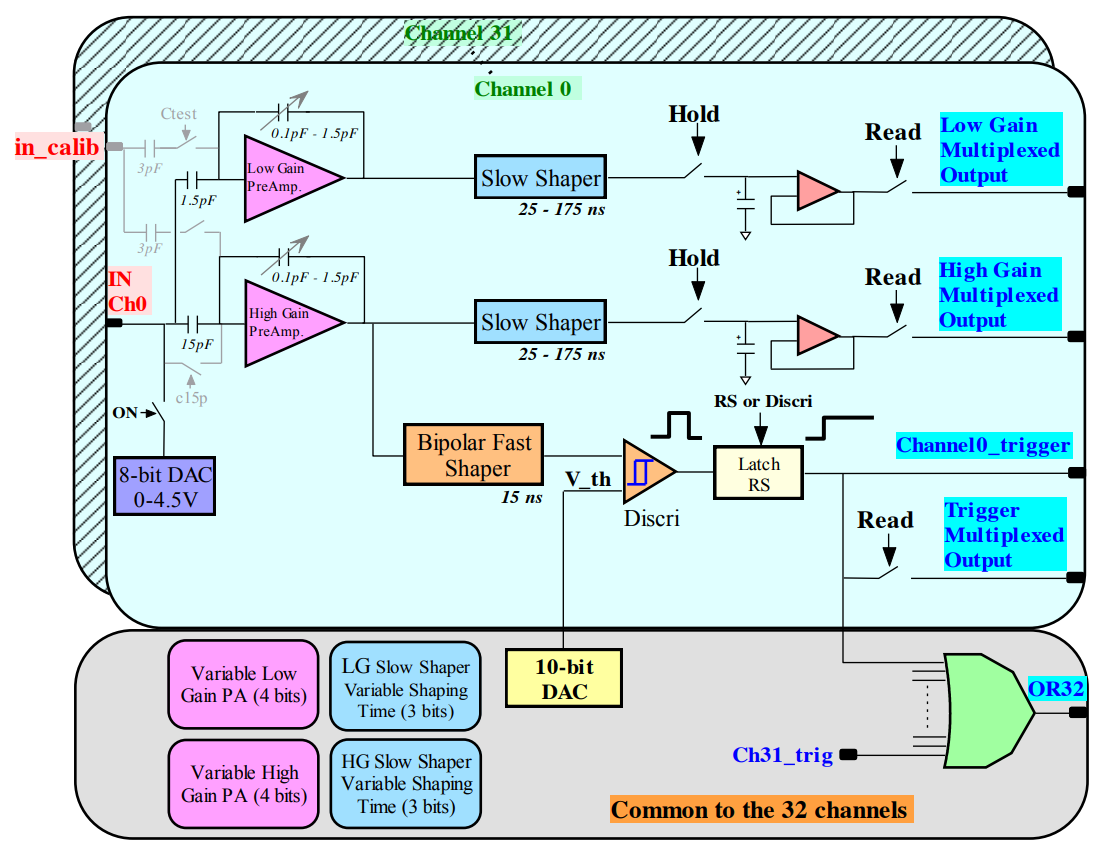
\includegraphics[width=12cm]{EASIROCCircuitDiagram.PNG}
\end{center}
\caption{EASIROC回路概略}
\end{figure}
各デバイスを通った信号の出力波形は、EASIROCモジュールのProbe出力を観察するとわかる。Fast ShaperはSelf Trigger用なので、今回は(おそらく)使わない。Trigger信号に合わせてShaperの波高の一番高いところが読み出されているのがわかる。Trigger信号とShaperの立ち上がりがきちんと合うかどうかはケーブルの長さやDelayモジュールによって操作できる。
\begin{figure}[h]
\begin{tabular}{cccc}
\begin{minipage}[t]{0.25\hsize}
\begin{center}
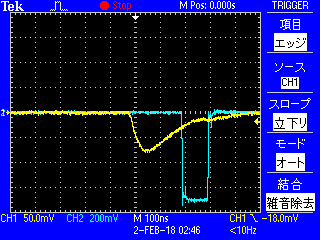
\includegraphics[width=4cm]{preamp.BMP}
\end{center}
\caption{Pre-Amp}
\end{minipage}
\begin{minipage}[t]{0.25\hsize}
\begin{center}
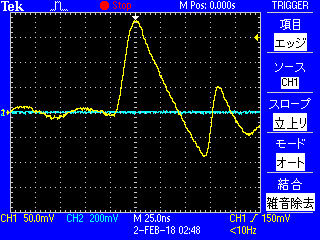
\includegraphics[width=4cm]{fastshaper.BMP}
\end{center}
\caption{Fast Shaper}
\end{minipage}
\begin{minipage}[t]{0.25\hsize}
\begin{center}
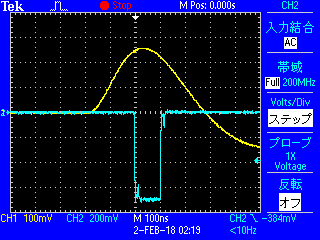
\includegraphics[width=4cm]{slowshaper.BMP}
\end{center}
\caption{Slow Shaper}
\end{minipage}
\begin{minipage}[t]{0.25\hsize}
\begin{center}
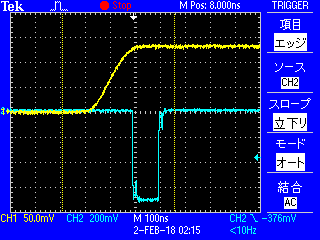
\includegraphics[width=4cm]{slowshaperhold.BMP}
\end{center}
\caption{holdしたSlow Shaper}
\end{minipage}
\end{tabular}
\end{figure}
\subsection{データ収集の方法}
詳しくはマニュアル参照。\\
EASROCボードのそれぞれのチャンネルが何をするものかは、User Guideの1章を参照すること。
2章には、EASIROCボードの制御法が記されている。EASIROCボードと交信し、制御するソフトウェアの名前もeasirocである。各種パラメータを反映したり、データ取得モードの指令もここから行う。印加するHVの制御及びモニタリングはudpで行う。ターミナルを2つ以上立ち上げて同時に操作するとよい。\\
easiroc IPアドレス(おそらく192.168.10.102) DAQmode(とりあえず3でOK)で特定のIPアドレスのEASIROCボードをそのDAQmodeで制御できる。多チャンネル読み出しなので、ReadSC\_Channnel1.txtでanalog outputから出すチャンネルを選び、ソフトウェアeasirocの指令2でそれを反映すると、オシロスコープで波形を観察できる。\\
User Guideに簡単な操作法が記されているが、ボード仕様書にはさらに細かい情報が載っているので、困ったら参照すること。
